\section[PCA]{PCA}
En el código se hizo uso tanto del cálculo manual de los PCA como de los métodos incluidos en la biblioteca Sckit.

\subsection[Manual]{Método manual}
Para el método manual se siguieron los siguientes pasos:
\begin{itemize}
    \item[1.] Se normaliza el dataset
    \begin{itemize}
        \item[1.1.] Cálculo de la media
        \item[1.2.] Cálculo de le desviación estándar
        \item[1.3.] Cálculo de valores estandarizados
    \end{itemize}
    \item[2.] Cálculo de la covarianza
    \item[3.] Cálculo de los eigenvalores y eigenvectores
    \begin{itemize}
        \item[3.1.] Ordenamiento de los eigenvalores y eigenvectores
        \item[3.2.] Suma acumulativa de eigenvalores y eigenvectores
    \end{itemize}
    \item[4.] Cálculo de componentes principales
    \begin{itemize}
        \item[4.1.] Cálculo de componentes mínimos
        \item[4.2.] Cálculo de los PCA a partir de los cálculos anteriores
    \end{itemize}
    \item[5.] Transformación del espacio original del dataset al de los PCA (bidimensional)
\end{itemize}

\subsubsection[Valores]{valores}
A continuación se detallarán los resultados en los pasos más relevantes:
\begin{itemize}
    \item \textbf{Media}: Indican el valor representativo o el valor ubicado a la mitad del rango de valores donde se encuentran la mayoría de datos.
    \item \textbf{Desviación estándar}: Este valor se puede interpretar como el número que indica qué tan alejado está el punto a analizar con respecto a la media.
    \item \textbf{Valor estandarizado}: Este valor corresponde a su reflejo en una distribución normal estandarizada.
    \item \textbf{Covarianza}: Este número indica la tendencia a variar de manera paralela, en este caso, de los distintos datos del dataset.
    \item \textbf{Eigenvalores y eigenvectores}: Estos valores nos indica la relación matemática entre las dimensiones del dataset y nos ayuda, posteriormente, al cálculo de los PCA.
\end{itemize}

\subsubsection[Relación de los PCA]{Diagrama de relación de Componentes Principales}
A continuación se muestra el diagrama de los PCA calculados y su relación con las dimensiones originales:
\begin{center}
    \begin{figure}[!h]
        \centering
        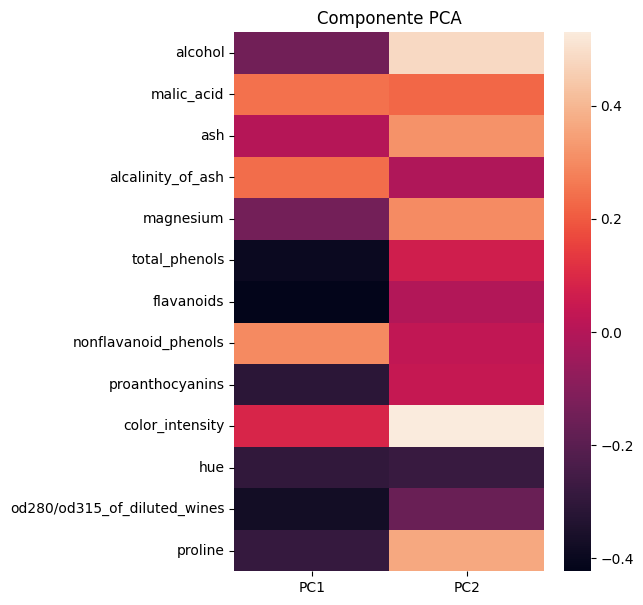
\includegraphics[scale=0.67]{PCACorrelation.png}
        \caption{Diagrama de relación de los componentes calculados con las dimensiones originales}
    \end{figure}
\end{center}

En ese diagrama se observa que las columnas representan a los 2 componentes calculados anteriormente y, por la escala, aquellos con el tono correspondiente al valor 0.0 o cercanos son aquellos que no tienen una relación directa con el componente.
Así, para el PCA 1 se mantienen relacionadas las siguientes dimensiones:
\begin{itemize}
    \item Positivas
    \begin{itemize}
        \item malic\_acid
        \item alcalinity\_of\_ash
        \item nonflavanoid\_phenols
    \end{itemize}                                                                                                                                                                                                                                                                                                                                                                                                                                                                                                                                                                    
    \item Negativas
    \begin{itemize}
        \item alcohol
        \item magnesium
        \item total\_phenols
        \item flavanoids
        \item proanthocyanins
        \item hue
        \item od280/od315\_of\_diluted\_wines
        \item proline
    \end{itemize}
    \item Cercanas ninguna
    \begin{itemize}
        \item ash
        \item color\_intensity
    \end{itemize}
\end{itemize}
Y para el PCA 2:
\begin{itemize}
    \item Positivas
    \begin{itemize}
        \item alcohol
        \item malic\_acid
        \item ash
        \item magnesium
        \item color\_intensity
        \item proline
    \end{itemize}                                                                                                                                                                                                                                                                                                                                                                                                                                                                                                                                                                    
    \item Negativas
    \begin{itemize}
        \item hue
        \item od280/od315\_of\_diluted\_wines
    \end{itemize}
    \item Cercanas ninguna
    \begin{itemize}
        \item alcalinity\_of\_ash
        \item total\_phenols
        \item flavanoids
        \item nonflavanoid\_phenols
        \item proanthocyanins
    \end{itemize}
\end{itemize}
Con estos resultados podemos decretar que con estos dos componentes se mantiene la relación entre las dimensiones originales y los calculados gracias a que los componentes cumplen complementariamente con la corespondencia.

\subsubsection[Transformación]{Transformación}
Una vez calculados los PCA, los datos se llevan al espacio bidimensional. La gráfica correspondiente se muestra a continuación:

\begin{center}
    \begin{figure}[!ht]
        \centering
        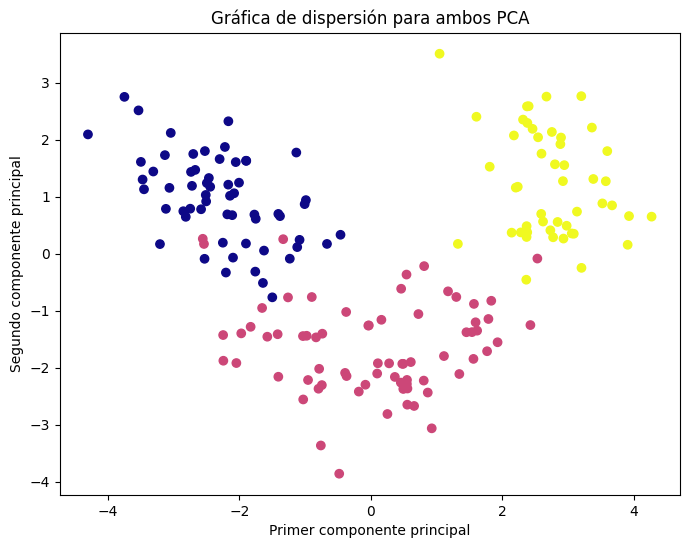
\includegraphics[scale=0.67]{Manual_PCA_Scatter.png}
        \caption{Diagrama de dispersión de los datos originales con las PCA calculadas}
    \end{figure}
\end{center}
\vskip 10cm

\subsection[Automatico]{Método automático}
Este método está incluido en la \href{https://scikit-learn.org/stable/modules/generated/sklearn.decomposition.PCA.html}{biblioteca de Scikit} y se tiene que importar explícitamente.

Los resultados que arroja son los siguientes:
